\documentclass[
	% -- opções da classe memoir --
	12pt,				% tamanho da fonte
	openright,			% capítulos começam em pág ímpar (insere página vazia caso preciso)
	oneside,			% para impressão em verso e anverso. Oposto a oneside
	a4paper,			% tamanho do papel. 
	% -- opções da classe abntex2 --
	%chapter=TITLE,		% títulos de capítulos convertidos em letras maiúsculas
	%section=TITLE,		% títulos de seções convertidos em letras maiúsculas
	%subsection=TITLE,	% títulos de subseções convertidos em letras maiúsculas
	%subsubsection=TITLE,% títulos de subsubseções convertidos em letras maiúsculas
	% -- opções do pacote babel --
	english,			% idioma adicional para hifenização
	french,				% idioma adicional para hifenização
	spanish,			% idioma adicional para hifenização
	brazil				% o último idioma é o principal do documento
	]{abntex2}
 
% ----------------------------------------------------------
% CONFIGURAÇÃO DO DOCUMENTO
% ----------------------------------------------------------

% ----------------------------------------------------------
% IMPORTAÇÃO DE PACOTES
% ----------------------------------------------------------

% ---
% PACOTES BASICOS
% ---
\usepackage{lmodern}			% Usa a fonte Latin Modern			
\usepackage[T1]{fontenc}		% Selecao de codigos de fonte.
\usepackage[utf8]{inputenc}		% Codificacao do documento (conversão automática dos acentos)
\usepackage{lastpage}			% Usado pela Ficha catalográfica
\usepackage{indentfirst}		% Indenta o primeiro parágrafo de cada seção.
\usepackage{color}				% Controle das cores
\usepackage{graphicx}			% Inclusão de gráficos
\usepackage{microtype} 			% para melhorias de justificação


%------------------------------------------------
%\usepackage[brazil]{babel}
\usepackage{dsfont}
\usepackage{multirow}
\usepackage{multicol}
\usepackage{colortbl}
\usepackage{url}
%\usepackage{abntcite}
\usepackage{algorithm}
\usepackage{algorithmic}
%\usepackage{alg}
%\usepackage{hyperref}
\usepackage{caption} 
\usepackage{subcaption} % for subfigures

% para usar os comentários nos algoritmos
% conforme definido mais abaixo em:
% \renewcommand{\algorithmiccomment}[1]{\hfill\eqparbox{}{\# #1}}
\usepackage{eqparbox}

% exibe somente capitulo, seção e subseção
\setcounter{tocdepth}{2}

\newcommand{\abreviarEN}[2][abreviatura]{(\abrv[#1 -- #2]{#1}, do inglês \textit{#2})}

%------------------------------------------------



% ---
% PACOTES ADICIONAIS, USADOS APENAS NO ÂMBITO DO MODELO CANÔNICO DO abnteX2
% ---
\usepackage{lipsum}				% para geração de dummy text

% ---
% PACOTES DE CITAÇÕES
% ---
\usepackage[brazilian,hyperpageref]{backref}	 % Paginas com as citações na bibl
\usepackage[alf]{abntex2cite}	% Citações padrão ABNT

% ---
% PACOTES ADICIONADOS POR CEPHAS
% ---
\usepackage{float}
\usepackage{amssymb,amsmath}
\usepackage{pdfpages}
\usepackage{acronym}

% --- 
% CONFIGURAÇÕES DE PACOTES
% --- 

% Configurações do pacote backref
% Usado sem a opção hyperpageref de backref
\renewcommand{\backrefpagesname}{Citado na(s) página(s):~}
% Texto padrão antes do número das páginas
\renewcommand{\backref}{}
% Define os textos da citação
\renewcommand*{\backrefalt}[4]{
	\ifcase #1 %
		Nenhuma citação no texto.%
	\or
		Citado na página #2.%
	\else
		Citado #1 vezes nas páginas #2.%
	\fi}%
% ---

% utilizando o todo notes para deixar comentários
\setlength {\marginparwidth }{2cm}
\usepackage[colorinlistoftodos]{todonotes}
%\usepackage[disable,colorinlistoftodos]{todonotes}
\newcommand{\duvida}[1]{\todo[color=yellow, inline, textcolor=black]{\texttt{Duvida:} #1}}
\newcommand{\lembrete}[1]{\todo[color=lightgray, inline, textcolor=black]{\texttt{Lembrete:} #1}}
\newcommand{\parafazer}[1]{\todo[color=green, inline, textcolor=black]{\texttt{Para Fazer:} #1}}

% Macros para indicar modificações no texto
\usepackage[normalem]{ulem}
\newcommand{\removido}[1]{\textcolor{red}{\sout{#1}}}
\newcommand{\novo}[1]{\textcolor{blue}{#1}}

% Macros para remover as modificações de texto na versão final
% comentar acima e descomentar abaixo na versão final
% \newcommand{\removido}[1]{}
% \newcommand{\novo}[1]{#1}
% \renewcommand*{\sout}{}

% Para poder ter tabelas com colunas de largura auto-ajustável
\usepackage{tabularx}

% Redefinicao de instrucoes
\floatname{algorithm}{Algoritmo}
\renewcommand{\algorithmicrequire}{\textbf{Entrada:}}
\renewcommand{\algorithmicensure}{\textbf{Saída:}}
\renewcommand{\algorithmicend}{\textbf{fim}}
\renewcommand{\algorithmicif}{\textbf{se}}
\renewcommand{\algorithmicthen}{\textbf{então}}
\renewcommand{\algorithmicelse}{\textbf{senão}}
\renewcommand{\algorithmicfor}{\textbf{para}}
\renewcommand{\algorithmicforall}{\textbf{para todo}}
\renewcommand{\algorithmicdo}{\textbf{faça}}
\renewcommand{\algorithmicwhile}{\textbf{enquanto}}
\renewcommand{\algorithmicloop}{\textbf{loop}}
\renewcommand{\algorithmicrepeat}{\textbf{repetir}}
\renewcommand{\algorithmicuntil}{\textbf{até que}}
\renewcommand{\algorithmiccomment}[1]{\hfill\eqparbox{}{\# #1}}

% Definicao da lista de simbolos
% \simb[entrada na lista de simbolos]{simbolo}:
% Escreve o simbolo no texto e uma entrada na lista de simbolos.
% Se o parametro opcional e omitido, usa-se o parametro obrigatorio.
\newcommand{\simb}[2][]
{%
	\ifthenelse{\equal{#1}{}}
	{\addcontentsline{los}{simbolo}{#2}}
	{\addcontentsline{los}{simbolo}{#1}}#2
}
% Para aceitar comandos com @ (at) no nome
\makeatletter 
% \listadesimbolos: comando que imprime a lista de simbolos
\newcommand{\listadesimbolos}
{
	\pretextualchapter{Lista de símbolos}
	{\setlength{\parindent}{0cm}
	\@starttoc{los}}
}
% Como a entrada sera impressa
\newcommand\l@simbolo[2]{\par #1}
\makeatother

% Definicao da lista de abreviaturas e siglas
% \abrv[entrada na lista de simbolos]{abreviatura}:
% Escreve a sigla/abreviatura no texto e uma entrada na lista de abreviaturas e siglas.
% Se o parametro opcional e omitido, usa-se o parametro obrigatorio.
\newcommand{\abrv}[2][]
{%
	\ifthenelse{\equal{#1}{}}
	{\addcontentsline{loab}{abreviatura}{#2}}
	{\addcontentsline{loab}{abreviatura}{#1}}#2
}
% Para aceitar comandos com @ (at) no nome
\makeatletter 
% \listadeabreviaturas: comando que imprime a lista de abreviaturas e siglas
\newcommand{\listadeabreviaturas}
{
	\pretextualchapter{Lista de abreviaturas e siglas}
	{\setlength{\parindent}{0cm}
	\@starttoc{loab}}
}
% Como a entrada sera impressa
\newcommand\l@abreviatura[2]{\par #1}
\makeatother

% \listofalgorithms: comando que imprime a lista de algoritmos
\renewcommand{\listalgorithmname}{Lista de algoritmos}


% ----------------------------------------------------------
% ELEMENTOS DA CAPA
% ----------------------------------------------------------
% ---
% Informações de dados para CAPA e FOLHA DE ROSTO
% ---
\titulo{Título da Dissertação}
\autor{Vinicius Pereira Santana}
\local{Natal-RN}
\data{2023}
\orientador{Dr. Prof. Ramon dos Reis Fontes}
%\coorientador{titulo e nome do seu coorientador}
\instituicao{%
  Universidade Federal do Rio Grande do Norte -- UFRN
  \par
  Instituto Metrópole Digital -- IMD
  \par
  Programa de Pós-Graduação em Tecnologia da Informação -- PPgTI}
\tipotrabalho{Dissertação de Mestrado}
% O preambulo deve conter o tipo do trabalho, o objetivo, 
% o nome da instituição e a área de concentração 
\preambulo{Dissertação de Mestrado apresentada ao Programa de Pós-graduação em Tecnologia da Informação da Universidade Federal do Rio Grande do Norte como requisito para a obtenção do grau de Mestre em Tecnologia da Informação.}
% ---
% ----------------------------------------------------------
% APARENCIA DO PDF FINAL 
% ----------------------------------------------------------
% Configurações de aparência do PDF final

% alterando o aspecto da cor azul
\definecolor{blue}{RGB}{41,5,195}

% informações do PDF
\makeatletter
\hypersetup{
     	%pagebackref=true,
		pdftitle={\@title}, 
		pdfauthor={\@author},
    	pdfsubject={\imprimirpreambulo},
	    pdfcreator={LaTeX with abnTeX2},
		pdfkeywords={abnt}{latex}{abntex}{abntex2}{trabalho acadêmico}, 
		colorlinks=true,       		% false: boxed links; true: colored links
    	linkcolor=blue,          	% color of internal links
    	citecolor=blue,        		% color of links to bibliography
    	filecolor=magenta,      		% color of file links
		urlcolor=blue,
		bookmarksdepth=4
}
\makeatother
% --- 

% --- 
% Adicionado para evitar warning de Uppercase
% --- 
\pdfstringdefDisableCommands{\let\uppercase\relax}

% --- 
% Espaçamentos entre linhas e parágrafos 
% --- 

% O tamanho do parágrafo é dado por:
\setlength{\parindent}{1.3cm}

% Controle do espaçamento entre um parágrafo e outro:
\setlength{\parskip}{0.2cm}  % tente também \onelineskip

% ---
% compila o indice
% ---
\makeindex
% ---


% ----------------------------------------------------------
% ----------------------------------------------------------
% Início do documento
% ----------------------------------------------------------
% ----------------------------------------------------------
\begin{document}

% Seleciona o idioma do documento (conforme pacotes do babel)
\selectlanguage{brazil}
% Retira espaço extra obsoleto entre as frases.
\frenchspacing 

% ----------------------------------------------------------
% ELEMENTOS PRÉ-TEXTUAIS
% ----------------------------------------------------------
\pretextual

% ----------------------------------------------------------
% CAPA
% ----------------------------------------------------------
% Mude para usar capa limpa ou customizada (Includes/Capa.tex)
% Capa
% Proteção externa do trabalho e sobre a qual se imprimem as informações indispensáveis 
% à sua identificação.

%Capa modificada para o PPgSW

% Especificação da capa
\begin{titlingpage}
	\begin{center}
		% Cabeçalho (não deve ser modificado)
		% Contém o brasão da Universidade, o logotipo do Departamento, além dos dados
		% relacionados à vinculação do aluno (Universidade, Centro, Departamento e Curso)
		\hspace*{-1.5cm}
		\begin{minipage}{2.2cm}
			\begin{center}
				
\includegraphics[width=2.25cm, height=2.68cm]{Imagens/Brasao-UFRN.jpg}
			\end{center}
		\end{minipage}
		\begin{minipage}{12.5cm}
			\begin{center}
			%	\begin{espacosimples}
					{\small \ \\
                       \textsc{Universidade Federal do Rio Grande do Norte}		   			\\
							  \textsc{Instituto Metrópole Digital}					\\
							  \textsc{Programa de Pós-graduação em Tecnologia da Informação}	\\
                       \textsc{Mestrado Profissional em Tecnologia da Informação}}   				\\
			%	\end{espacosimples}
			\end{center}
		\end{minipage}
		\begin{minipage}{2.cm}
			\begin{center}
				
\includegraphics[width=1.8cm, height=1.5cm]{Imagens/Logotipo-IMD}
			\end{center}
		\end{minipage}
			
		\vspace{6cm}
						
		% Título do trabalho
		{\setlength{\baselineskip}%
		{1.3\baselineskip}
		{\LARGE \textbf{Uma Proposta de Sistema Anti-UAV de Baixo Custo para o Combate a Invasores em Áreas Restritas}}}
			
		\vspace{3cm}
			
		% Nome do aluno (autor)
		{\large \textbf{Vinicius Pereira Santana}}
						
		\vspace{6cm}
		
		% Local da instituição onde o trabalho deve ser apresentado e ano de entrega do mesmo
	Natal-RN\\Outubro de 2023 % exemplo: agosto de 2018
	\end{center}
\end{titlingpage}

% não usar o \imprimircapa, usar a capa customizada
%\imprimircapa



% ----------------------------------------------------------
% FOLHA DE ROSTO
% ----------------------------------------------------------
% Folha de rosto (o * indica que haverá a ficha bibliográfica)
\imprimirfolhaderosto

% ----------------------------------------------------------
% FICHA BIBLIOGRAFICA
% ----------------------------------------------------------
%% ---
% Inserir a ficha bibliografica
% ---

% Após defender seu mestrado vc deve seguir os passos no sigaa para submissão da sua dissertação à UFRN. A biblioteca lhe enviará via Sigaa a ficha bibliográfica em PDF. Se tiver tudo certo, importe ela como foi feito abaixo.
%
%\begin{fichacatalografica}
   % 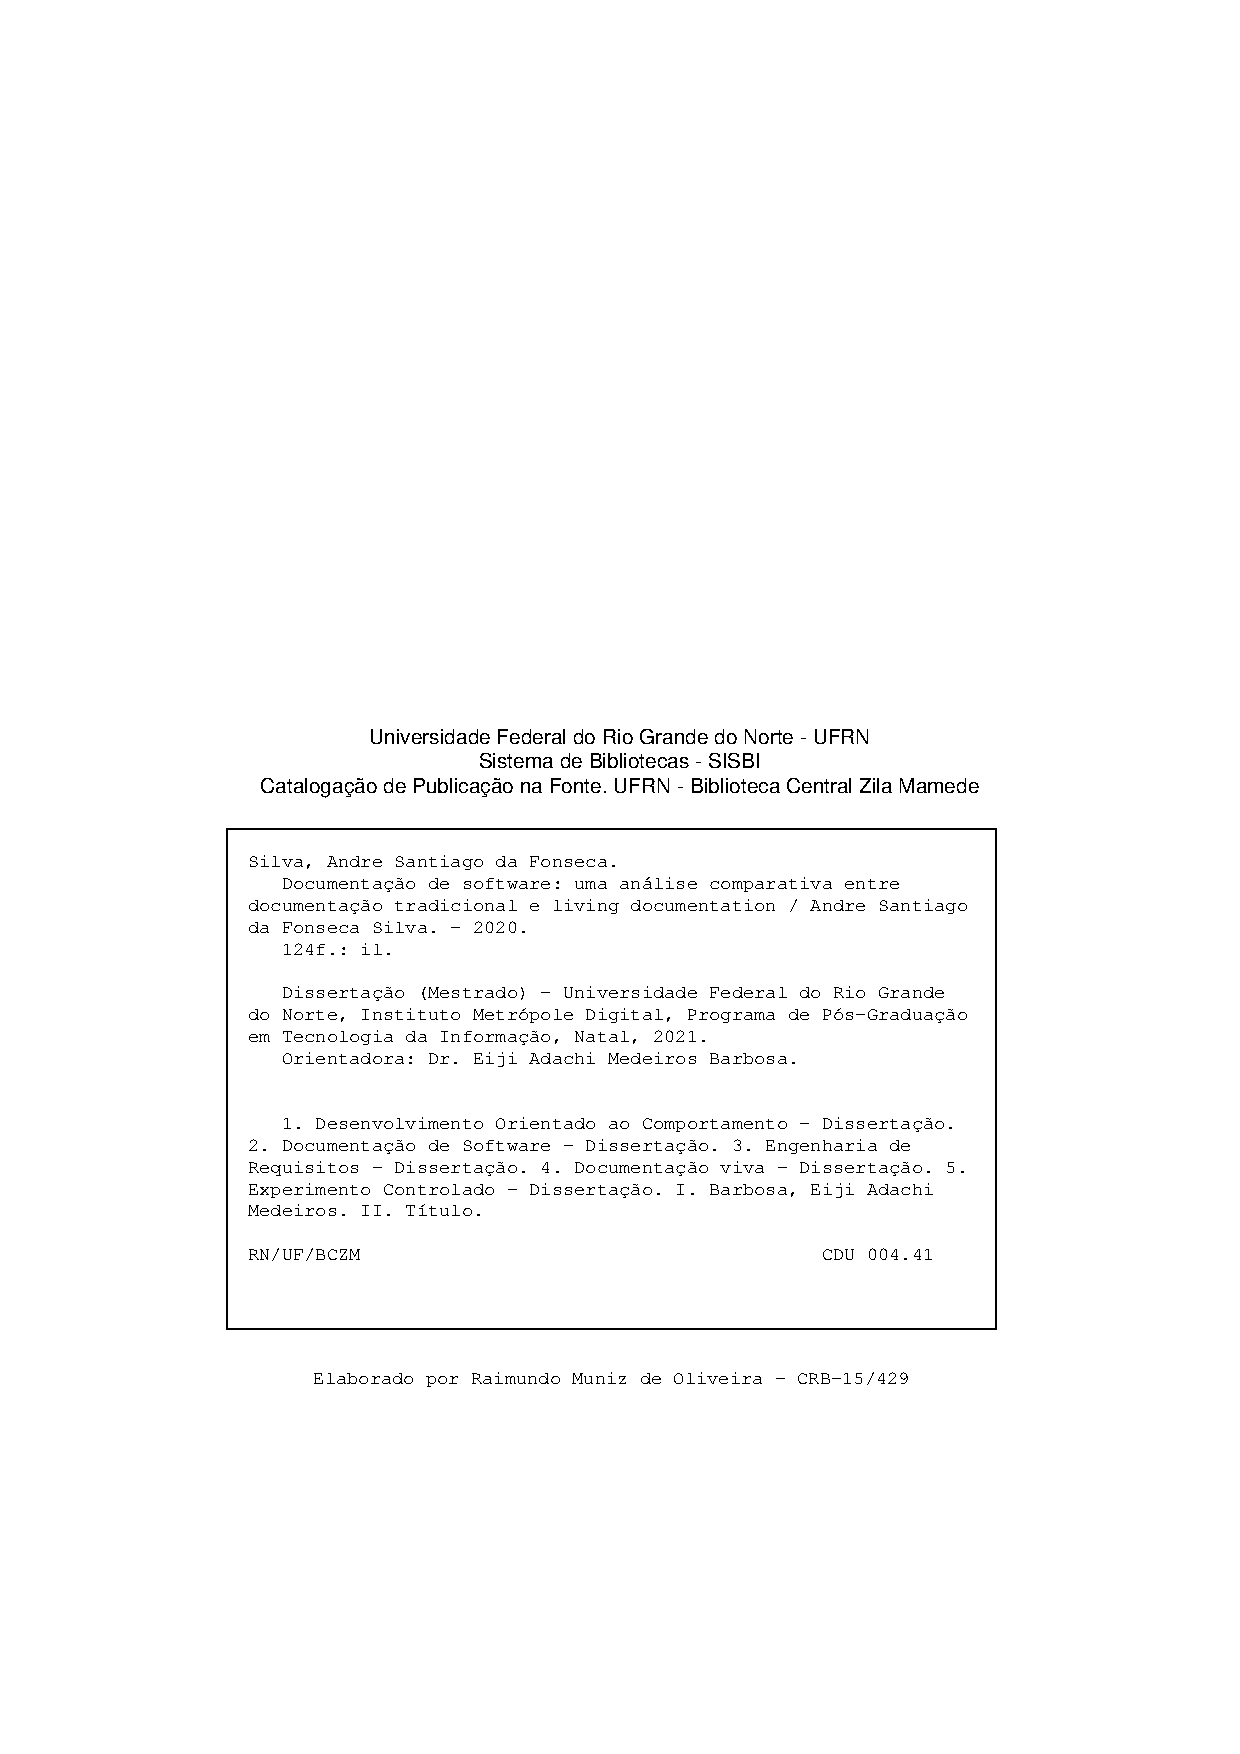
\includepdf[pages=-]{Includes/ficha.pdf}
%\end{fichacatalografica}

% ----------------------------------------------------------
% ERRATA
% ----------------------------------------------------------
%\begin{errata}
%Elemento opcional da \citeonline[4.2.1.2]{NBR14724:2011}. Exemplo:

%Se não for usar, deixe o input no "main" comentado  

\vspace{\onelineskip}

FERRIGNO, C. R. A. \textbf{Tratamento de neoplasias ósseas apendiculares com
reimplantação de enxerto ósseo autólogo autoclavado associado ao plasma
rico em plaquetas}: estudo crítico na cirurgia de preservação de membro em
cães. 2011. 128 f. Tese (Livre-Docência) - Faculdade de Medicina Veterinária e
Zootecnia, Universidade de São Paulo, São Paulo, 2011.

\begin{table}[htb]
\center
\footnotesize
\begin{tabular}{|p{1.4cm}|p{1cm}|p{3cm}|p{3cm}|}
  \hline
   \textbf{Folha} & \textbf{Linha}  & \textbf{Onde se lê}  & \textbf{Leia-se}  \\
    \hline
    1 & 10 & auto-conclavo & autoconclavo\\
   \hline
\end{tabular}
\end{table}

\end{errata}
% ---

% ----------------------------------------------------------
% FOLHA DE APROVACAO
% ----------------------------------------------------------
%% Folha de aprovação
\begin{folhadeaprovacao}
	%\setlength{\ABNTsignthickness}{0.4pt}
	%\setlength{\ABNTsignwidth}{10cm}
	
	% Informações gerais acerca do trabalho 
	% (nome do autor, título, instituição à qual é submetido e natureza)
	\noindent 
	Dissertação de Mestrado sob o título \textit{Título da Dissertação} apresentada por \textbf{Fulano de Tal} e aceita pelo Programa de Pós-graduação em Tecnologia da Informação da Universidade Federal do Rio Grande do Norte, sendo aprovada por todos os membros da banca examinadora abaixo especificada:
		
	% Membros da banca examinadora e respectivas filiações
	\assinatura
	{
		Prof. Dr. Professor Sicrano  			                  \\
		{\small Presidente}											          \smallskip\\ 
		{\footnotesize
			IMD -- Instituto Metrópole Digital		   \\ %apenas um exemplo
		  	UFRN -- Universidade Federal do Rio Grande do Norte %apenas um exemplo
		}
   }
      
   \assinatura
	{
		Prof. Dr. Examinador 1               \\
		{\small Examinador}											          \smallskip\\ 
		{\footnotesize
		    DCC –- Departamento de Ciência da Computação\\
			UFXX -- Universidade Federal de XX		   \\
		}
   }   
   
   \assinatura
	{
		Profa. Dra. Examinadora 2       \\
		{\small Examinador}											          \smallskip\\ 
	    {\footnotesize
			DI –- Departamento de Informática
			UFX -- Universidade Federal de XX		   \\
		}
	}
	
	\vfill
	
	\begin{center}
		Natal-RN, 28 de Dezembro de 2020.
	\end{center}
\end{folhadeaprovacao}


\begin{folhadeaprovacao}

  \begin{center}
    {\ABNTEXchapterfont\large\imprimirautor}

    \vspace*{\fill}\vspace*{\fill}
    \begin{center}
      \ABNTEXchapterfont\bfseries\Large\imprimirtitulo
    \end{center}
    \vspace*{\fill}
    
    \hspace{.45\textwidth}
    \begin{minipage}{.5\textwidth}
        \imprimirpreambulo
    \end{minipage}%
    \vspace*{\fill}
   \end{center}
        
   Trabalho aprovado. \imprimirlocal, 28 de Dezembro de 2020:

   \assinatura{\textbf{\imprimirorientador} \\ Orientador} 
   \assinatura{\textbf{Dr. Examinador 1} \\ Examinador}
   \assinatura{\textbf{Dra. Examinadora 2	} \\ Examinador}
   
   %\assinatura{\textbf{Professor} \\ Convidado 4}
      
   \begin{center}
    \vspace*{0.5cm}
    {\large\imprimirlocal}
    \par
    {\large\imprimirdata}
    \vspace*{1cm}
  \end{center}
  
\end{folhadeaprovacao}


% ----------------------------------------------------------
% DEDICATORIA
% ----------------------------------------------------------
%% Dedicatória

\chapter*{}
\vspace{15cm}
\begin{flushright}
	Dedico este trabalho a ...
\end{flushright}
\begin{flushright}
	Também dedico a....
\end{flushright}


% ----------------------------------------------------------
% AGRADECIMENTOS
% ----------------------------------------------------------
%% Agradecimentos
\chapter*{Agradecimentos}

Agradeço a ...

% ----------------------------------------------------------
% EPIGRAFE
% ----------------------------------------------------------
%% Epígrafe (citação seguida de indicação de autoria)

\chapter*{}
\vspace{15cm}
\begin{flushright}
	\textit
	{
		Citação inspiradora.
	}\medskip\\ 
	Autor da citação.
\end{flushright}

% ----------------------------------------------------------
% RESUMO
% ----------------------------------------------------------
% Resumo em língua vernácula
\begin{center}
	{\Large{\textbf{Título do trabalho}}}
\end{center}

\vspace{1cm}

\begin{flushright}
	Autor: Nome do Aluno\\
	Orientador: Prof. Dr. Orientador\\ 
\end{flushright}

\vspace{1cm}

\begin{center}
	\Large{\textsc{\textbf{Resumo}}}
\end{center}

\noindent O resumo deve apresentar de forma concisa os pontos relevantes de um texto, fornecendo uma visão rápida e clara do conteúdo e das conclusões do trabalho. O texto, redigido na forma impessoal do verbo, é constituído de uma seqüência de frases concisas e objetivas e não de uma simples enumeração de tópicos, não ultrapassando 500 palavras, seguido, logo abaixo, das palavras representativas do conteúdo do trabalho, isto é, palavras-chave e/ou descritores. Por fim, deve-se evitar, na redação do resumo, o uso de parágrafos (em geral resumos são escritos em parágrafo único), bem como de fórmulas, equações, diagramas e símbolos, optando-se, quando necessário, pela transcrição na forma extensa, além de não incluir citações bibliográficas.

\noindent De uma forma geral, um bom resumo deve conter: \\
- Uma introdução, que deve ser usada para apresentar o tema do texto, incluindo o problema a ser resolvido. \\
- Depois, abordar objetivo geral do artigo/dissertação/tese\\
- Apresentar uma descrição simples da metodologia e da proposta; \\
- Descrever os principais resultados obtidos (mesmo que sejam parciais)

\noindent\textit{Palavras-chave}: Palavra-chave 1, Palavra-chave 2, Palavra-chave 3.


% ----------------------------------------------------------
% RESUMO
% ----------------------------------------------------------
% Resumo em língua estrangeira (em inglês Abstract, em espanhol Resumen, em francês Résumé)
\begin{center}
	{\Large{\textbf{Título em inglês}}}
\end{center}

\vspace{1cm}

\begin{flushright}
	Autor: Vinicius Pereira Santana\\
	Supervisor 1: Prof. Dr. Ramon dos Reis Fontes
    Supervisor 2: Prof. Dr. Roger
\end{flushright}

\vspace{1cm}

\begin{center}
	\Large{\textsc{\textbf{Abstract}}}
\end{center}

%\noindent O resumo em língua estrangeira (em inglês \textit{Abstract}, em espanhol \textit{Resumen}, em francês \textit{Résumé}) é uma versão do resumo escrito na língua vernácula para idioma de divulgação internacional. Ele deve apresentar as mesmas características do anterior (incluindo as mesmas palavras, isto é, seu conteúdo não deve diferir do resumo anterior), bem como ser seguido das palavras representativas do conteúdo do trabalho, isto é, palavras-chave e/ou descritores, na língua estrangeira. Embora a especificação abaixo considere o inglês como língua estrangeira (o mais comum), não fica impedido a adoção de outras linguas (a exemplo de espanhol ou francês) para redação do resumo em língua estrangeira.

\noindent\textit{Keywords}: Keyword 1, Keyword 2, Keyword 3.

% ----------------------------------------------------------
% LISTA DE ILUSTRACOES
% ----------------------------------------------------------
\chapter*{}
% ---
% inserir lista de ilustrações
% ---
\pdfbookmark[0]{\listfigurename}{lof}
\listoffigures*
\cleardoublepage
% ---

% ----------------------------------------------------------
% LISTA DE TABELAS
% ----------------------------------------------------------
% ---
% inserir lista de tabelas
% ---
\pdfbookmark[0]{\listtablename}{lot}
\listoftables*
\cleardoublepage
% ---

% ----------------------------------------------------------
% LISTA DE ABREVIATURAS E SIGLAS
% ----------------------------------------------------------


% Lista de abreviaturas e siglas
\listadeabreviaturas

% ----------------------------------------------------------
% LISTA DE SIMBOLOS
% ----------------------------------------------------------
% Lista de símbolos
\listadesimbolos

% ----------------------------------------------------------
% LISTA DE ALGORITMOS
% ----------------------------------------------------------
% Lista de algoritmos (se houver)
% Devem ser incluídos os pacotes algorithm e algorithmic
\listofalgorithms


% ----------------------------------------------------------
% SUMARIO
% ----------------------------------------------------------
% ---
% inserir o sumario
% ---
\pdfbookmark[0]{\contentsname}{toc}
\tableofcontents*
\cleardoublepage
% ---

% ----------------------------------------------------------
% Lista de ToDO
% ----------------------------------------------------------
\listoftodos
        
% ----------------------------------------------------------
% ----------------------------------------------------------
% ELEMENTOS TEXTUAIS
% ----------------------------------------------------------
% ----------------------------------------------------------
\textual

% Introdução
\chapter{Introdução}
\label{cap:capitulo1}
% label do capítulo para usar como referência no texto
% O Capítulo~\ref{cap:capitulo1} fala sobre

A introdução deve dar ao leitor o posicionamento da tese e a motivação suficiente para a leitura da tese, esclarecendo:
\begin{itemize}
	\item A natureza do problema cuja resolução se descreve (uma palhinha do problema);
	\item Uma indicação dos métodos usados para atacar o problema;
	\item As contribuições do trabalho e sua relevância para fazer progredir o estado da arte. Se for uma tese, aqui se coloca a hipótese de pesquisa, a tese, e como ela será demonstrada durante o texto;
	\item A forma como a tese está estruturada (estrutura do texto).
\end{itemize}

Uma dica para a montagem de uma tese ou monografia é responder as seguintes perguntas, cada uma em um parágrafo:
\begin{itemize}
	\item \textbf{O que fez?}: O que se propõe, o que se trabalhou, ``Propomos...'';
	\item \textbf{Como fez?}: Técnicas, metodologia de trabalho, ``Para tal...'';
	\item \textbf{Por que?}: Quais as motivações e justificativas do trabalho. A motivação inclui se faz parte de um projeto maior, o fato do problema não ter solução, e/ou qual a história que o levou a trabalhar nisso. A justificativa não é obrigatória, mas pode motivar o leitor;
	\item \textbf{Quanto vale?}: Quais as contribuições do trabalho. Inclui hipótese, tese,  e resultados principais (técnicas, métodos novos, produtos, publicações);
	\item \textbf{Para quem?} Quais as aplicações que se beneficiarão do seu trabalho, para quê será (ou poderá ser) usado - como parte de um projeto;
	\item \textbf{Como está?} Estrutura do texto. Evite escrever coisas obvias (como ``na Introdução, introduzimos...'', ``na conclusão, concluímos''). Coloque texto informativo, que acrescente o saber de quem lê (como ``na seção 2 será mostrado por que \textbf{wavelets} podem ser usadas para estabilizar corrente'').
\end{itemize}

Uma observação importante é não colocar ``Objetivos'' nos trabalhos finais, pois não são mais objetivos, uma vez que você os atingiu. Neste caso, estes viram contribuições. Os ``Objetivos'' são mais utilizados para qualificações e projetos de pesquisa, que ainda não foi desenvolvidos. Tomar cuidado também para colocar objetivos factíveis (porque será um problema se não os cumprir...).

\section{Problema de pesquisa}
\label{sec:problema}

\section{Motivação}


\section{Objetivos}

A pesquisa realizada é baseada nos objetivos geral e específicos que são apresentados a seguir.

\subsection{Objetivo Geral}

\subsection{Objetivos Específicos}

\begin{itemize}
    \item Objetivo 1;
    \item Objetivo 2;
    \item Objetivo 3;
    \item Objetivo 4;
    \item Objetivo 5;
\end{itemize}

\section{Solução Proposta}
\label{sec:solucao}

\section{Metodologia}
\label{sec:metodologia}

\section{Estrutura do trabalho}

Os capítulos desta dissertação estão organizados da seguinte forma:

\textbf{Capítulo~\ref{cap:capitulo1} -} Introduz o problema, apresenta a motivação e os objetivos do trabalho.

\textbf{Capítulo~\ref{cap:capitulo2} -} Apresenta o referencial teórico sobre as tecnologias relacionadas a solução proposta na pesquisa.

\textbf{Capítulo~\ref{cap:capitulo3} -} Apresenta trabalhos relacionados a pesquisa e problemas existentes.

\textbf{Capítulo~\ref{cap:capitulo4} -} Apresentação da arquitetura proposta, com detalhamento das camadas.

\textbf{Capítulo~\ref{cap:capitulo5} -} Demonstra os resultados obtidos após utilização do protótipo.

\textbf{Capítulo~\ref{cap:capitulo6} -} Considerações finais, breve apresentação dos resultados obtidos, limitações e dificuldades encontradas e trabalhos futuros. 


% Capítulo 2
%----------------------------------------------
\chapter{Referencial teórico}
\label{cap:capitulo2}
% label do capítulo para usar como referência no texto
%----------------------------------------------

Breve resumo do que será apresentado no capítulo.

 %----------------------------------------------
\section{Dicas para utilização do \LaTeX}
%----------------------------------------------

Parágrafo de introdução.

%----------------------------------------------
\subsection{Dicas gerais}
%----------------------------------------------

\textbf{Não} utilizar aspas duplas, exemplo "aspas".  Utilizar duas crases para abrir aspas (\`{}\`{}) e duas aspas simples (\textquotesingle\textquotesingle) para fechar. Resultado fica ``assim''. 

No \LaTeX, o til (\~{}) pode ser utilizado para significar um espaço em branco sem permitir a quebra de linha neste local. Ou seja, quando utilizado desta forma ``\verb|Tabela~\ref{tab:exemplo}|'', não vai haver quebra de linha entre a palavra ``Tabela'' e o seu número ``1'', por exemplo. Desta forma, é recordável a utilização em todas as referências cruzadas (tabelas, figuras, algoritmos, quadros, etc) (e.g., \verb|~\ref{}|) e também em citações (e.g., \verb|~\cite{}|).


%----------------------------------------------
\subsection{Referências a figuras, tabelas, seções}
\label{sec:usarLabels}
%----------------------------------------------

Utilizar a tag \verb|\label{}| para adicionar nomes aos elementos e depois usar a tag \verb|\ref{}| para referenciar. Exemplo referenciando a Seção~\ref{sec:usarLabels}. 

%----------------------------------------------
\subsection{ToDo Notes}
%----------------------------------------------

Utilizar as macros de notas. 

\verb|\parafazer{}|
\parafazer{Atividade/Ações/Escritas que ainda precisam ser realizadas.}

\verb|\duvida{}|
\duvida{Deixe sua duvida registrada aqui.}

\verb|\lembrete{}|
\lembrete{Deixar um comentário, uma observação.}

Não é necessário apagar ou comentar as notas manualmente para que elas não apareçam no PDF, basta adicionar ``disable'' na inserção do pacote.

\begin{verbatim}
Arquivo -> dissertacao.tex 
Linha ->   \usepackage[disable,colorinlistoftodos]{todonotes}.
\end{verbatim}

%---------------------------------------------- 
\subsection{Notas de rodapé}
%----------------------------------------------

Texto\footnote{https://www.google.com} é um mecanismo de automação utilizado
	    
%----------------------------------------------
\subsection{Figuras}
%----------------------------------------------

A Figura~\ref{fig:figuraTeste} exibe ...

O código de inserção das figuras deve \textbf{sempre} estar localizado abaixo da primeira referência a esta. O próprio \LaTeX vai posicionar a imagem. Utilizar a tag \verb|[!htb]|.

% exemplo de figura
\begin{figure}[!htb]
    \centering
    \includegraphics[width=\textwidth]{example-image-a}
    % pode tem ser definido o tamanho da figura 
    %width = largura
    %height = altura
    %\includegraphics[width=10cm,height=10cm]{Imagens/FiguraTeste.png}
    \caption{Legenda da figura} 
    % label é utilizado para referenciar a figura no texto
    % A Figura~\ref{fig:figuraTeste} exibe ...
    \label{fig:figuraTeste}
\end{figure}


Para referenciar a figura inteira, utilizar \verb|~\ref{fig:2imagens}|, ex. Figura~\ref{fig:2imagens}. Para referenciar somente A, utilizar \verb|~\ref{fig:labelFigA}|, ex. Figura~\ref{fig:labelFigA} e somente B utilizar \verb|~\ref{fig:labelFigB}|, ex. Figura~\ref{fig:labelFigB}.

\begin{figure}[!htp]
        \centering
        \begin{subfigure}[t]{0.4\textwidth}
                \includegraphics[width=\textwidth]{example-image-a}
                \caption{} % se quiser adicionar descrição ao lado de (a)
                \label{fig:labelFigA}
        \end{subfigure}       
        \begin{subfigure}[t]{0.4\textwidth}
                \includegraphics[width=\textwidth]{example-image-b}
                \caption{}
                \label{fig:labelFigB}
        \end{subfigure}
        %\vspace{-2\baselineskip} % ajustar a posição da legenda, se for necessário. Negativo aproxima da imagem, Positivo afasta
        \caption{Duas imagens e somente uma legenda}\label{fig:2imagens}
\end{figure}


\begin{figure}
\centering
  \begin{subfigure}[t]{.4\textwidth}
    \centering
    \includegraphics[width=\textwidth]{example-image-a}
    \caption{\textbf{Schnitt}: $A \cup B$: Element liegt in $A$ \textbf{oder} in $B$.}
  \end{subfigure}
  %\hfill % adicionar espaço entre as imagens
  \begin{subfigure}[t]{.4\textwidth}
    \centering
    \includegraphics[width=\textwidth]{example-image-b}
    \caption{\textbf{Vereinigung}: $A \cap B$: Element liegt in $A$ \textbf{und} in $B$.}
  \end{subfigure}
  \begin{subfigure}[t]{.4\textwidth}
    \centering
    \includegraphics[width=\textwidth]{example-image-c}
    \caption{\textbf{Differenz}: $A \setminus B$: Element liegt in $A$ \textbf{nicht} in $B$. (\textit{A ohne B})}
  \end{subfigure}
  %\hfill % adicionar espaço entre as imagens
  \begin{subfigure}[t]{.4\textwidth}
    \centering
    \includegraphics[width=\textwidth]{example-image-a}
    \caption{\textbf{Symmetrische Differenz}: $A \Delta B$: Element liegt \textbf{entweder} in $A$ oder in $B$.}
  \end{subfigure}
  \caption{Quatro imagens lado a lado}\label{fig:4imagens} 
\end{figure}



\begin{figure}
\centering
\begin{subfigure}[b]{.45\linewidth}
\includegraphics[width=\linewidth]{example-image-a}
\caption{A mouse}\label{fig:mouse}
\end{subfigure}
\begin{subfigure}[b]{.45\linewidth}
\includegraphics[width=\linewidth]{example-image-b}
\caption{A gull}\label{fig:gull}
\end{subfigure}
\begin{subfigure}[b]{.45\linewidth}
\includegraphics[width=\linewidth]{example-image-c}
\caption{A tiger}\label{fig:tiger}
\end{subfigure}
\caption{Picture of animals}
\label{fig:animals}
\end{figure}

%----------------------------------------------
\subsection{Indicar alterações no texto.}
%----------------------------------------------

Utilize \verb|\removido{}| para marcar um texto antigo, que será removido. Exemplo, \removido{texto a ser removido na próxima revisão.} 

Utilize \verb|\novo{}| para marcar os novos textos inseridos depois de uma revisão. Exemplo, \novo{Colocar aqui os novos textos inseridos, facilitando assim as revisões futuras.} 

Exemplo de Algoritmo~\ref{alg:alg1}.

\begin{algorithm} % enter the algorithm environment
\caption{Nome do algoritmo} % give the algorithm a caption
\label{alg:alg1} % and a label for \ref{} commands later in the document
\begin{algorithmic}[1] % enter the algorithmic environment
                       % [1] insere numeração de linhas
    \REQUIRE $n \geq 0 \vee x \neq 0$
    \ENSURE $y = x^n$ \COMMENT{some comment here}
    \STATE $y \Leftarrow 1$
    \IF{$n < 0$}
        \STATE $X \Leftarrow 1 / x$
        \STATE $N \Leftarrow -n$
    \ELSE
        \STATE $X \Leftarrow x$
        \STATE $N \Leftarrow n$
    \ENDIF
    \WHILE{$N \neq 0$}
        \IF{$N$ is even}
            \STATE $X \Leftarrow X \times X$
            \STATE $N \Leftarrow N / 2$
        \ELSE  [$N$ is odd]
            \STATE $y \Leftarrow y \times X$
            \STATE $N \Leftarrow N - 1$
        \ENDIF
    \ENDWHILE
    \FOR{xxxx}
        \STATE $X \Leftarrow x$
    \ENDFOR
\end{algorithmic}
\end{algorithm}



\begin{algorithm}
\caption{Calculate $y = x^n$}
\label{alg1}
\begin{multicols}{2}
\begin{algorithmic}[1]
  \REQUIRE $n \geq 0 \vee x \neq 0$
  \ENSURE $y = x^n$
  \STATE $y \Leftarrow 1$
  \IF{$n < 0$}
  \STATE $X \Leftarrow 1 / x$
  \STATE $N \Leftarrow -n$
  \ELSE
  \STATE $X \Leftarrow x$
  \STATE $N \Leftarrow n$
  \ENDIF
  \WHILE{$N \neq 0$}
  \IF{$N$ is even}
  \STATE $X \Leftarrow X \times X$
  \STATE $N \Leftarrow N / 2$
  \ELSE [$N$ is odd]
  \STATE $y \Leftarrow y \times X$
  \STATE $N \Leftarrow N - 1$
  \ENDIF
  \ENDWHILE
\end{algorithmic}
\end{multicols}
\end{algorithm}


% Capítulo 3
\chapter{Trabalhos relacionados}
\label{cap:capitulo3}
% label do capítulo para usar como referência no texto
% O Capítulo~\ref{cap:capitulo3} fala sobre


Algumas regras devem ser observadas na redação da dissertação/tese: 

\begin{itemize}
   \item ser claro, preciso, direto, objetivo e conciso, utilizando frases curtas e evitando ordens inversas desnecessárias;
   \item construir períodos com no máximo duas ou três linhas, bem como parágrafos com cinco linhas cheias, em média, e no máximo oito (ou seja, não construir parágrafos e períodos muito longos, pois isso cansa o(s) leitor(es) e pode fazer com que ele(s) percam a linha de raciocínio desenvolvida);
   \item a simplicidade deve ser condição essencial do texto; a simplicidade do texto não implica necessariamente repetição de formas e frases desgastadas, uso exagerado de voz passiva (como \textit{será iniciado}, \textit{será realizado}), pobreza vocabular etc. Com palavras conhecidas de todos, é possível escrever de maneira original e criativa e produzir frases elegantes, variadas, fluentes e bem alinhavadas;
   \item adotar como norma a ordem direta, por ser aquela que conduz mais facilmente o leitor à essência do texto, dispensando detalhes irrelevantes e indo diretamente ao que interessa, sem ``rodeios'' (verborragias);
   \item não começar períodos ou parágrafos seguidos com a mesma palavra, nem usar repetidamente a mesma estrutura de frase;
   \item desprezar as longas descrições e relatar o fato no menor número possível de palavras;
   \item recorrer aos termos técnicos somente quando absolutamente indispensáveis e nesse caso colocar o seu significado entre parênteses (ou seja, não se deve admitir que todos os que lerão o trabalho já dispõem de algum conhecimento desenvolvido no mesmo);
   \item dispensar palavras e formas empoladas ou rebuscadas, que tentem transmitir ao leitor mera ideia de erudição (até mesmo às vezes ilusória);
   \item não perder de vista o universo vocabular do leitor, adotando a seguinte regra prática: \textit{nunca escrever o que não se diria};
   \item termos coloquiais ou de gíria devem ser usados com extrema parcimônia (ou mesmo nem serem utilizados) e apenas em casos muito especiais, para não darem ao leitor a ideia de vulgaridade e descaracterizar o trabalho;
   \item ser rigoroso na escolha das palavras do texto, desconfiando dos sinônimos perfeitos ou de termos que sirvam para todas as ocasiões; em geral, há uma palavra para definir uma situação;
   \item encadear o assunto de maneira suave e harmoniosa, evitando a criação de um texto onde os parágrafos se sucedem uns aos outros como compartimentos estanques, sem nenhuma fluência entre si;
   \item ter um extremo cuidado durante a redação do texto, principalmente com relação às regras gramaticais e ortográficas da língua; geralmente todo o texto é escrito na forma impessoal do verbo, não se utilizando, portanto, de termos em primeira pessoa, seja do plural ou do singular.
\end{itemize}

Continuação do texto.


\section{Seção A}

Teste de tabela. Tabela~\ref{tab:TabelaSemSentido}, referência à tabela definida abaixo.

\begin{table}[!htb]
   \caption{Tabela sem sentido.}
   \centering
   \medskip
   \begin{tabular}{c|p{4cm}}
      \hline
      \textbf{Título Coluna 1} & \textbf{Título Coluna 2} \\
      \hline
      Texto curto & Texto mais extenso, que requer mais de uma linha \\
      \hline
   \end{tabular}
   \label{tab:TabelaSemSentido}
\end{table}



\subsection{Subseção X}


Texto a ser enumerado.

\begin{enumerate}
   \item Item 1
   \item Item 2, com nota explicativa\footnote{Nota explicativa}
   \item Item 3
\end{enumerate}


\subsection{Subseção Y}

Texto antes de equação.

\begin{equation}
   x = y + z
\end{equation}

Texto depois de equação.
% Capítulo 4
\chapter{Modelo proposto}
\label{cap:capitulo4}
% label do capítulo para usar como referência no texto
% O Capítulo~\ref{cap:capitulo4} fala sobre


\section{Seção A}

Teste para símbolo

\simb[$\lambda$ (algum símbolo)]{$\lambda$}


\section{Seção B}

Teste para abreviatura 

\abrv[UFRN -- Universidade Federal do Rio Grande do Norte]{UFRN}

\abrv[DIMAp -- Departamento de Informática e Matemática Aplicada]{DIMAp}

\abrv[PPgTI -- Programa de Pós-graduação em Tecnologia da Informação]{PPgTI}


% comando criado em dissertacao.tex
\abreviarEN[IoT]{Internet of Things}




% Capítulo 5
\chapter{Avaliação dos resultados ou \\ Resultados preliminares}
\label{cap:capitulo5}
% label do capítulo para usar como referência no texto
% O Capítulo~\ref{cap:capitulo5} fala sobre


\section{Seção A}

Seção A


\section{Seção A}

Alguns exemplos de citação: 

Na tese de Doutorado de Paquete \cite{PaquetePhD}, discute-se sobre algoritmos de busca local estocásticos aplicados a problemas de Otimização Combinatória considerando múltiplos objetivos. Por sua vez, o trabalho de \cite{KnowlesBoundedLebesgue}, publicado nos anais do IEEE CEC de 2003, mostra uma técnica de arquivamento também empregada no desenvolvimento de algoritmos evolucionários multi-objetivo, trabalho esse posteriormente estendido para um capítulo de livro dos mesmos autores \cite{KnowlesBoundedPareto}. Por fim, no relatório técnico de \citeonline{Jaszkiewicz}, fala-se sobre um algoritmo genético híbrido para problemas multi-critério, enquanto no artigo de jornal de Lopez \textit{et al.} \cite{LopezPaqueteStu} trata-se do \textit{trade-off} entre algoritmos genéticos e metodologias de busca local, também aplicados no contexto multi-critério e relacionado de alguma forma ao trabalho de Jaszkiewicz (\citeyear{Jaszkiewicz}).

Outros exemplos relacionados encontram-se em \cite{Silberschatz} (livro), \cite{DB2XML} (referência da Web) e \cite{Angelo} (dissertação de Mestrado).

\subsection{Subseção X}

Subseção X


\subsection{Subseção Y}

Subsection Y


\section{Seção C}

Seção C
% Considerações finais
\chapter{Considerações finais}
\label{cap:capitulo6}
% label do capítulo para usar como referência no texto
% O Capítulo~\ref{cap:capitulo6} fala sobre

As considerações finais formam a parte final (fechamento) do texto, sendo dito de forma resumida (1) o que foi desenvolvido no presente trabalho e quais os resultados do mesmo, (2) o que se pôde concluir após o desenvolvimento bem como as principais contribuições do trabalho, e (3) perspectivas para o desenvolvimento de trabalhos futuros, como listado nos exemplos de seção abaixo. O texto referente às considerações finais do autor deve salientar a extensão e os resultados da contribuição do trabalho e os argumentos utilizados estar baseados em dados comprovados e fundamentados nos resultados e na discussão do texto, contendo deduções lógicas correspondentes aos objetivos do trabalho, propostos inicialmente.


%-----------------------------
% para dissertação 
\section{Principais contribuições}
Texto.


\section{Limitações}
Texto.


\section{Trabalhos futuros}
Texto.
%-----------------------------

%-----------------------------
% para qualificação
\section{Cronograma de Trabalho}
Texto.


\section{Resultados Esperados}
Texto.
%-----------------------------


% ----------------------------------------------------------
% Finaliza a parte (textual) no bookmark do PDF
% para que se inicie o bookmark na raiz
% e adiciona espaço de parte no Sumário
% ----------------------------------------------------------
\phantompart

% ----------------------------------------------------------
% ELEMENTOS PÓS-TEXTUAIS
% ----------------------------------------------------------
\postextual

% ----------------------------------------------------------
% Referências bibliográficas
% ----------------------------------------------------------
\bibliography{referencias}

% ----------------------------------------------------------
% Apêndices
% ----------------------------------------------------------
% ---
% Inicia os apêndices
% ---
\begin{apendicesenv}

% Imprime uma página indicando o início dos apêndices
\partapendices
% ----------------------------------------------------------
\chapter{Titulo deste apêndice}
\label{apendice:apendice1}
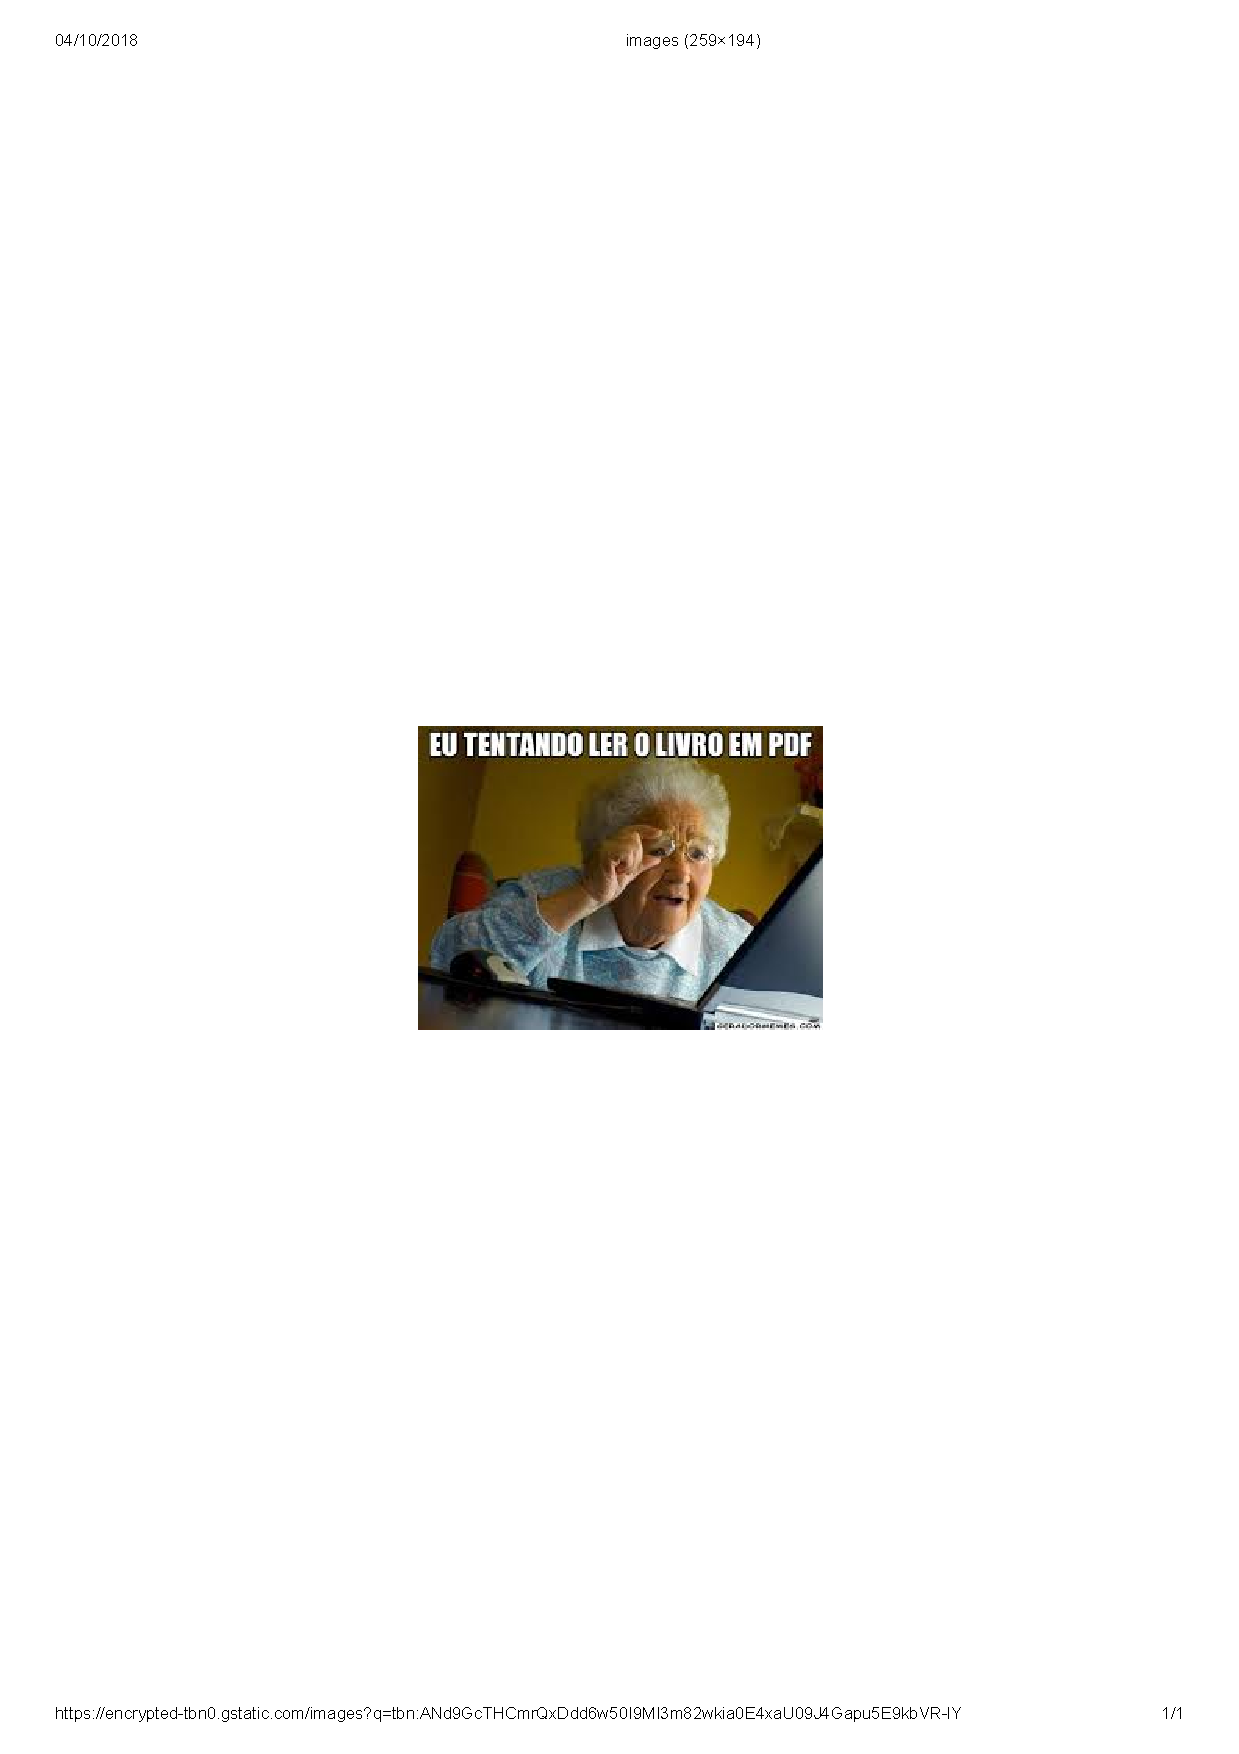
\includepdf[pages=-]{Anexos/exemplo.pdf}

\end{apendicesenv}

% ----------------------------------------------------------
% Anexos
% ----------------------------------------------------------
\begin{anexosenv}

% Imprime uma página indicando o início dos anexos
\partanexos

\chapter{Titulo deste anexo}
\label{anexo:anexo1}
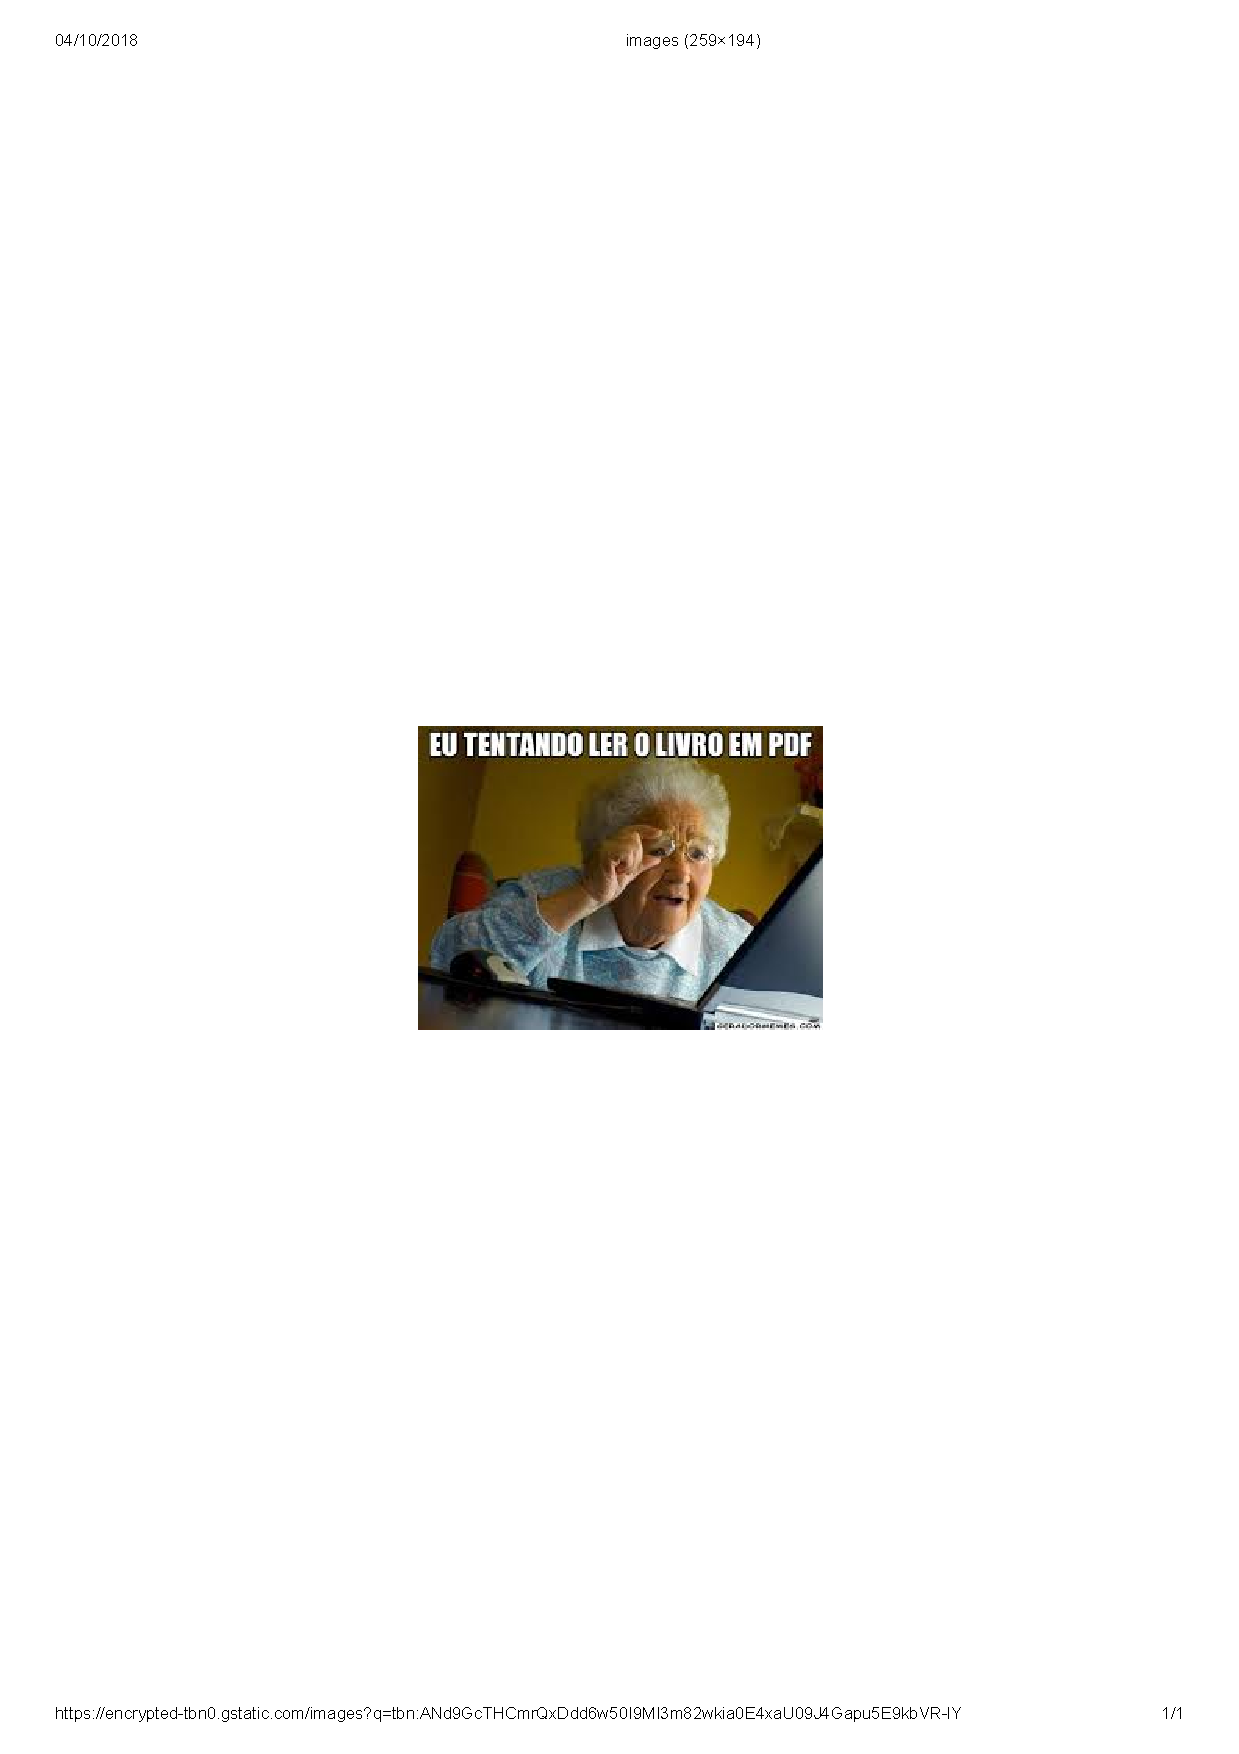
\includepdf[pages=-]{Anexos/exemplo.pdf}

\end{anexosenv}


%---------------------------------------------------------------------
% INDICE REMISSIVO
%---------------------------------------------------------------------

\phantompart
\printindex
%---------------------------------------------------------------------

\end{document}
